%!TEX root = ../aufgabenstellung.tex

\section{Einleitung}

Ein Logistikunternehmen möchte sein Verteilzentrum mit einer automatischen, roboterbasierten Paketsortieranlage ausstatten.
%In der Sortieranlage sollen eingehende Pakete auf die bereitstehenden Roboter aufgelegt werden, wobei die Pakete automatisch von einem Scanner erfasst und gewogen werden.
In der Sortieranlage werden eingehende Pakete auf die bereitstehenden Roboter aufgelegt und daraufhin automatisch von einem Scanner erfasst und gewogen.
Abhängig von den gescannten Informationen wird von der Sortieranlage ein Abwurfschacht bestimmt, in welchem der transportierende Roboter das Paket abwerfen soll.\footnote{Die Aufgabe basiert auf einer realen Paketsortieranlage, die unter anderem im folgenden Video dokumentiert ist: \url{https://www.youtube.com/watch?v=X_VLR7vU-8c}. Im Vergleich zum Video wurden die Abläufe in dieser Aufgabe vereinfacht. 
Das Fahrverhalten wurde an die deutsche Straßenverkehrsordnung angepasst.}

\begin{center}
	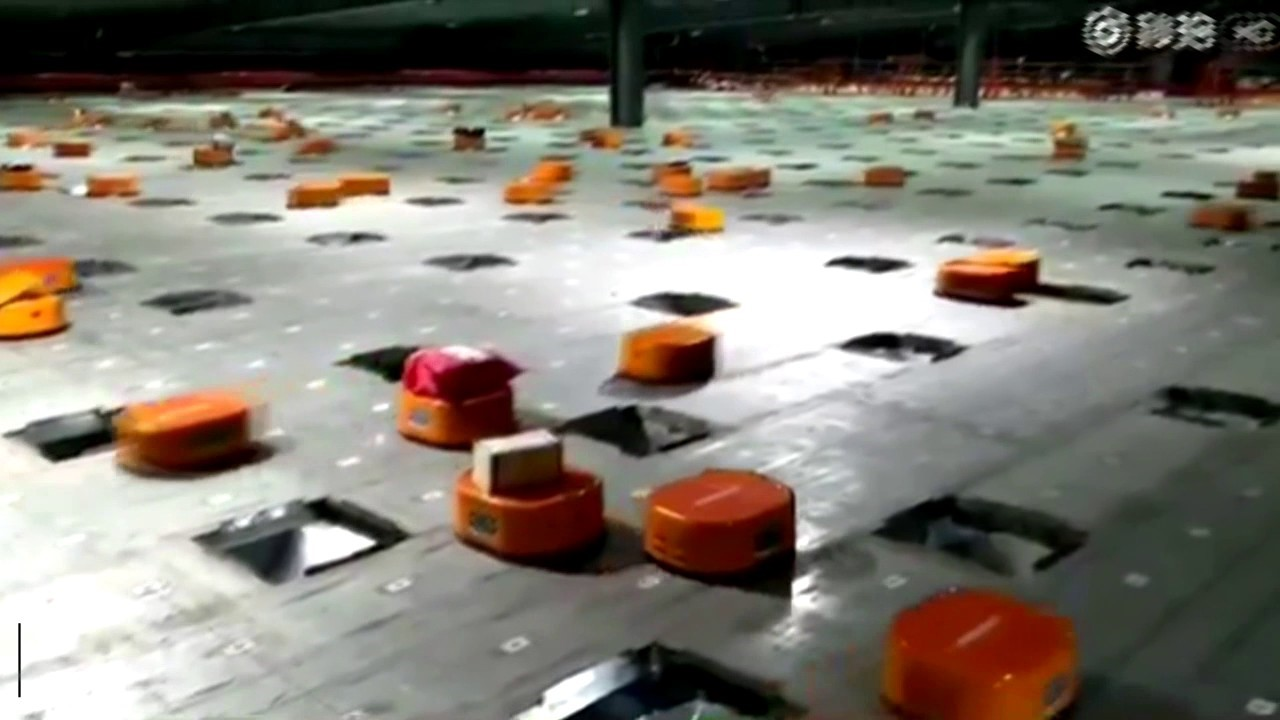
\includegraphics[width=0.9\textwidth]{robotvideo_img.jpg}
\end{center}

Die besondere Herausforderung an der Sortieranlage ist das Umsetzen von Verkehrsregeln für die autonom fahrenden Roboter, so dass diese ihre Pakete möglichst effizient transportieren und gleichzeitig Kollisionen untereinander oder mit Hindernissen vermeiden.

Im Rahmen eines zuvor durchgeführten Entwurfsprojektes wurde bereits eine Softwarearchitektur für die Roboter erarbeitet. Die Ergebnisse dieses objektorientierten Entwurfs, insbesondere die Struktur der Komponente \texttt{RobotControl} sowie die Spezifikation der enthaltenen Klassen und Methoden, werden im Entwurfsdokument \texttt{\red{Spezifikation.pdf}} bereitgestellt.

Um das kollisionsfreie Fahrverhalten gemäß der gegebenen Spezifikation sicherzustellen, soll in diesem Projekt ein \textbf{detaillierter Feinentwurf} für das Verhalten der Klasse \texttt{DriveSystem} durchgeführt werden.
Diese Klasse bestimmt das Fahrverhalten eines Roboters. Ihr Verhalten soll mithilfe eines \textbf{Statecharts} modelliert werden.
Das entstehende Statechart soll das Fahrverhalten eines Roboters so präzise modellieren, dass eine realistische Simulation und  Verifikation möglich ist.

Für die Modellierung und Simulation des Fahrverhaltens wird ein Tool bereitgestellt, welches in \texttt{\red{Toolhinweise.pdf}} genauer dokumentiert ist.

